\documentclass{article}

\usepackage{graphicx}
\usepackage[margin=2cm,a4paper]{geometry}
\usepackage{tcolorbox}
\tcbuselibrary{listings,skins}
\usepackage{listings}
\lstset{
  language=bash,
  basicstyle=\small\ttfamily,
  columns=flexible,
  breaklines=true,
  showstringspaces=false
}

\begin{document}

\title{Building IaaS infrastructures on the AWS Cloud}
\author{Saul Pierotti}
\date{\today}

\maketitle

\begin{abstract}
The abstract text goes here.
\end{abstract}

\section{General Description of the Infrastructure}
The demostrative infrastructure described in this project consists of an HTCcondor cluster of three nodes.
One node is configured as Master Node, while 2 nodes are configured as Worker Nodes.
The infrastructure can be easily expanded by replicating the Worker Nodes instances.

\section{Initialization of the instances on the AWS Cloud}
Worker Nodes and the Master Node were both built on the same base instance configuration.
The \texttt{t2.medium} instance type was used with a 50 Gb SSD as root storage.
The operating system choosen is Ubuntu Server 18.04.4 LTS.
The Master Node and the Worker Nodes were all instatiated in the same availability zone (\texttt{us-east-1a}), so that they would be able to communicate through private IPv4 adresses.
The security group for the instances was configured as follows:

\begin{figure}[!h]
	\center
	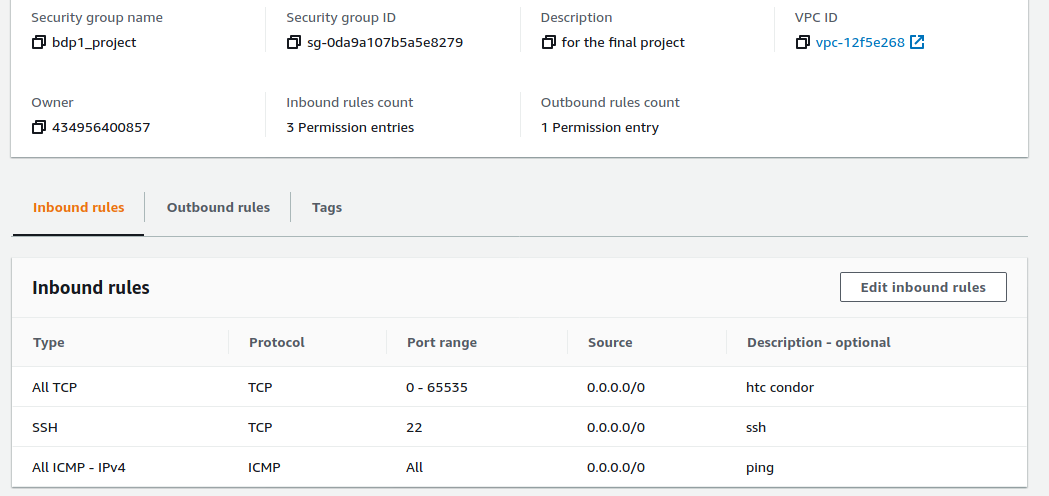
\includegraphics[width=\textwidth]{./images/security-group.png}
\end{figure}

The TCP ports 0-65535 required by HTCondor were open, as well as the ICMP ports for accepting incoming \texttt{ping} requests and the TCP port 22 for incoming \texttt{ssh} connections.

\section{Configuration of the Master Node}
The PS1 prompt of the Master Node was changed so to make the node easily identifiable from the command line.

\begin{figure}[!h]
	\center
	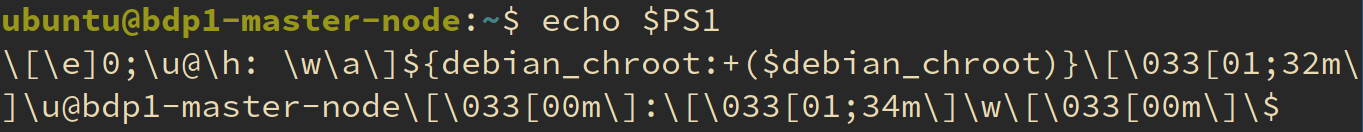
\includegraphics[width=\textwidth]{./images/master-ps1.png}
\end{figure}

HTCondor was then installed with the following commands:

\begin{lstlisting}
sudo su
wget -qO - https://research.cs.wisc.edu/htcondor/ubuntu/HTCondor-Release.gpg.key | apt-key add - # import the gpg key of HTCondor
echo "deb http://research.cs.wisc.edu/htcondor/ubuntu/8.8/bionic bionic contrib" >> /etc/apt/sources.list # add the repository
echo "deb-src http://research.cs.wisc.edu/htcondor/ubuntu/8.8/bionic bionic contrib" >> /etc/apt/sources.list
apt update
apt install htcondor
systemctl start condor # start and enable the condor service
systemctl enable condor
\end{lstlisting}

The correct proceeding of the installation and the start of the \texttt{condor} service where checked with the following commands:

\begin{figure}[!h]
	\center
	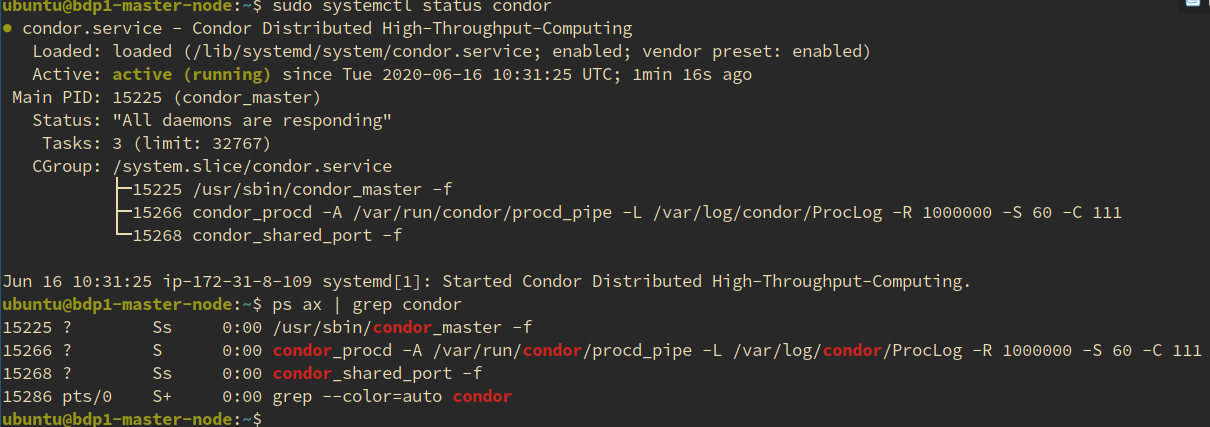
\includegraphics[width=\textwidth]{./images/condor_installed.png}
\end{figure}



\end{document}
